
\documentclass{beamer}

\usepackage{algpseudocode, color, colortbl}

\usepackage{hyperref}
\hypersetup{
    colorlinks=true,
    urlcolor=blue,
}

\usepackage{tikz, xcolor}

\usetheme{Montpellier}
\usecolortheme{rose}

% page numbers, from
% https://tex.stackexchange.com/questions/137022/how-to-insert-page-number-in-beamer-navigation-symbols
\expandafter\def\expandafter\insertshorttitle\expandafter{%
  \insertshorttitle\hfill%
  \insertframenumber\,/\,\inserttotalframenumber}

\definecolor{Gray}{gray}{0.8}
\newcolumntype{g}{>{\columncolor{Gray}}c}

\newcommand{\stanza}{ \\~\ }

\title{11. LP Duality and the Simplex Algorithm}
\subtitle{CPSC 535}
\author{Kevin A. Wortman}
\institute{ 
\includegraphics[height=2cm]{csuf-logo-cmyk} }
\date{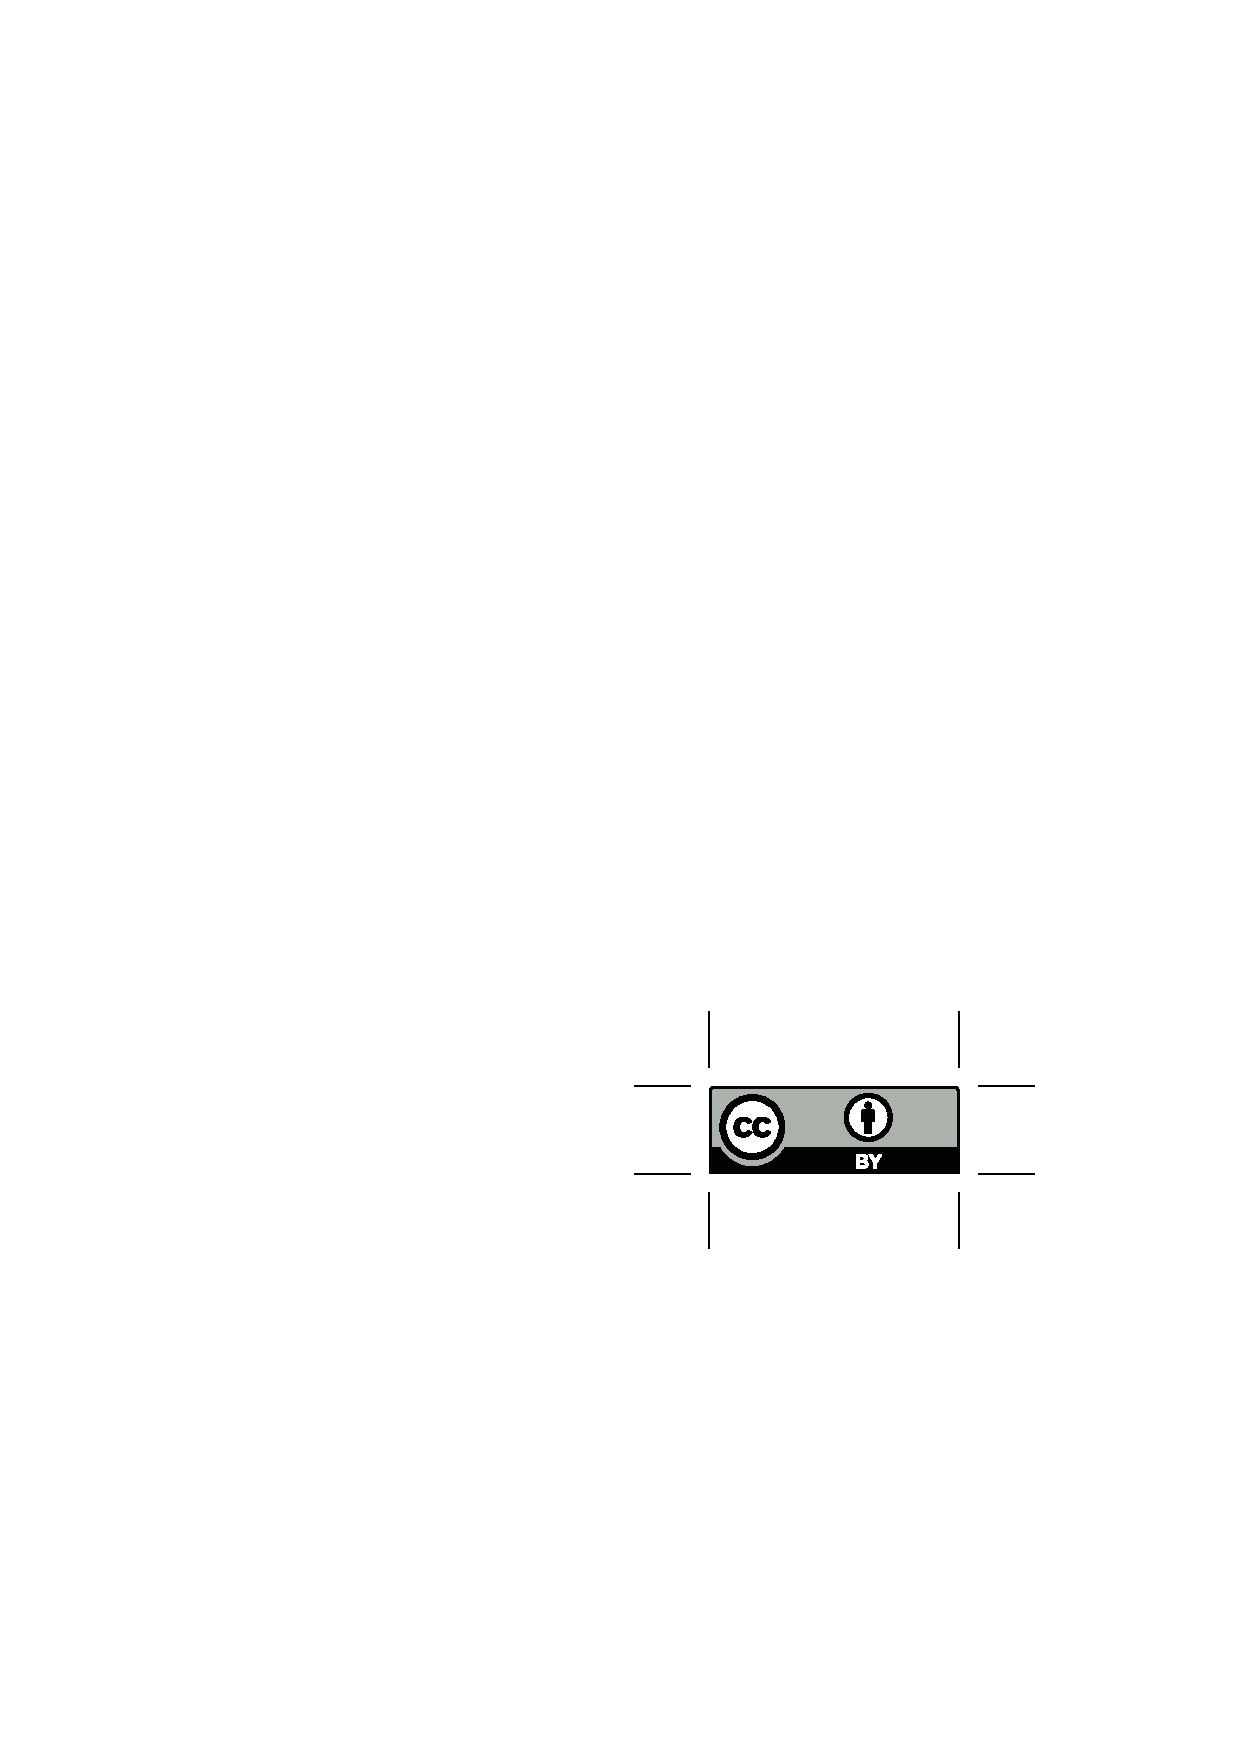
\includegraphics[height=14pt]{by} \\

{\tiny
This work is licensed under a
\href{http://creativecommons.org/licenses/by/4.0/}{Creative Commons Attribution 4.0 International License}.
}}

\begin{document}

\begin{frame}
  \titlepage
\end{frame}

\begin{frame} \frametitle{Recall: Standard Form}
standard form with $n$ variables and $m$ constraints:\stanza

maximize $c_1 x_1 + c_2 x_2 + \ldots + c_n x_n$ \\
subject to
\begin{eqnarray*}
a_{1,1} x_1 + a_{1,2} x_2 + \ldots + a_{1, n} x_{1, n} &\leq& b_1 \\
a_{2,1} x_1 + a_{2,2} x_2 + \ldots + a_{2, n} x_{2, n} &\leq& b_2 \\
\vdots & & \vdots \\
a_{m,1} x_1 + a_{m,2} x_2 + \ldots + a_{m, n} x_{m, n} &\leq& b_m \\
x_1, x_2, \ldots, x_n &\geq& 0
\end{eqnarray*}

\emph{variables:} $x_1, \ldots, x_n \in \mathbb{R}$ \\
\emph{objective function} defined by coefficients $c_1, \ldots, c_n \in \mathbb{R}$ \\
\emph{constraints} defined by coefficients $a_{i,j}, b_i \in \mathbb{R}$
\end{frame}

\begin{frame} \frametitle{Recall: Standard Form Matrix Notation}
\begin{itemize}
  \item more compact math notation
  \item collect:
  \begin{itemize}
    \item variables into vector $x=\langle x_1, \ldots, x_n \rangle$
    \item objective coefficients into vector $c=\langle c_1, \ldots, c_n\rangle$
    \item r.h.s. of inequalities into vector $b=\langle b_1, \ldots, b_m\rangle$
    \item $a_{i,j}$ coefficients into matrix $A$
  \end{itemize}
  \item LP can be written in terms of dot-product and matrix-vector multiplication
    as (and note the transpose $c^T$):
\end{itemize}
\vspace{.5cm}
maximize $c^T x$ \\
subject to
\begin{eqnarray*}
  Ax &\leq& b \\
  x &\geq& 0
\end{eqnarray*}
\end{frame}

\begin{frame} \frametitle{What is a Simplex?}
  \emph{simplex:} generalization of a triangle to arbitrary dimensions

  \begin{center}
  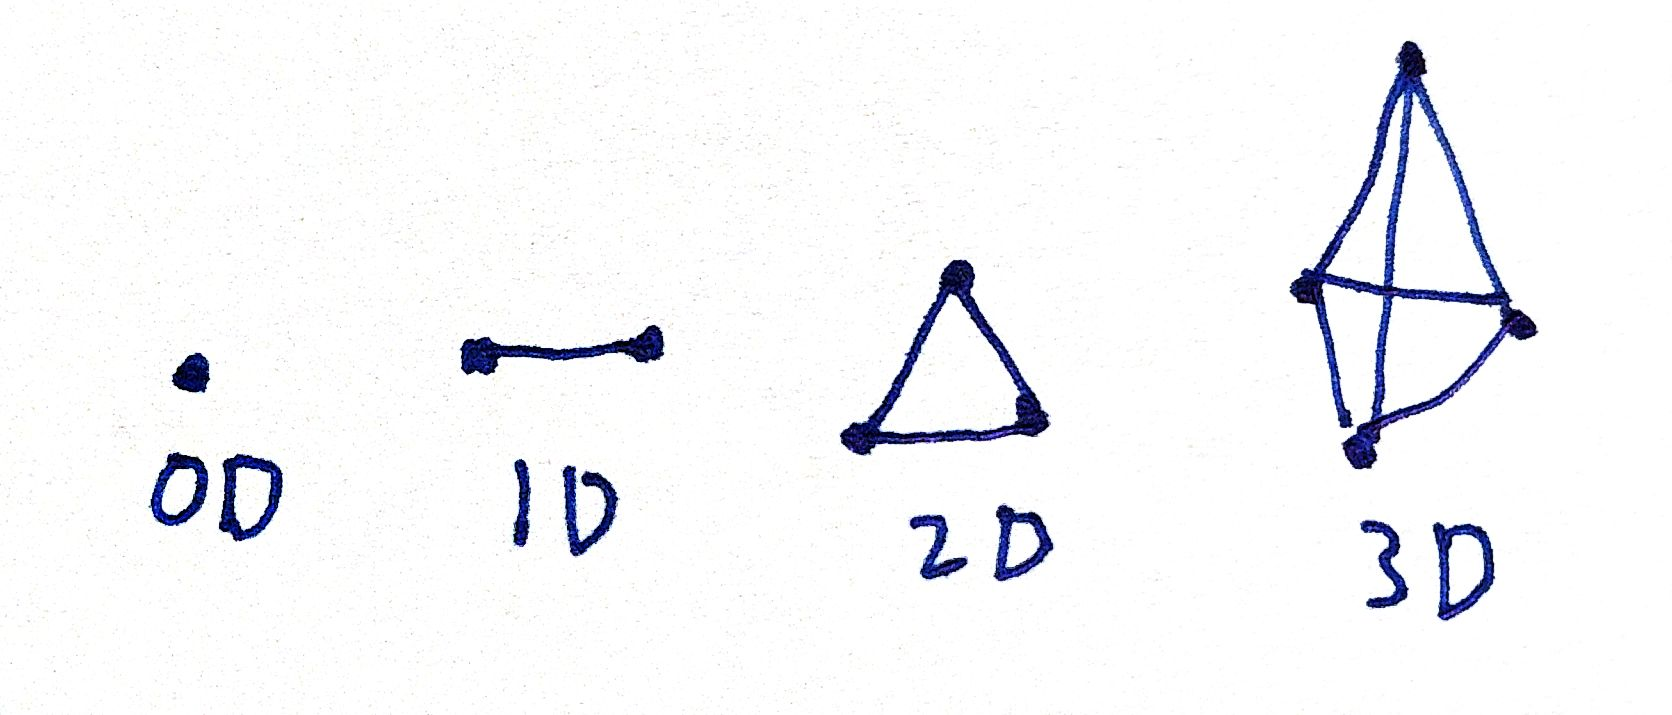
\includegraphics[width=4in]{simplices.jpg}
\end{center}
\end{frame}

\begin{frame} \frametitle{Slack Form}
\emph{duality:} the simplex algorithm views one LP in two ways,
\begin{enumerate}
  \item standard form
  \item \emph{slack form}
\end{enumerate}
\begin{itemize}
  \item standard form: constraint says l.h.s $\leq$ r.h.s.
  \item $\Rightarrow$ the difference or ``slack'' between l.h.s. and r.h.s.
    is $\geq 0$
  \item \emph{slack form:} constraint says l.h.s. $+$ \textbf{slack} $=$ r.h.s.
  \item increasing objective $=$ decreasing slack
  \item introduce one new \emph{basic variable} to represent slack in each constraint
  \item (pre-existing variables are \emph{nonbasic})
  \item $z$ = value of objective function
  \item don't bother writing ``maximize'' or ``subject to''
\end{itemize}
\end{frame}

\begin{frame} \frametitle{Standard versus Slack Form}
\begin{columns}
\begin{column}{.5\textwidth}
  maximize $x_1 + 2x_2 - \frac{1}{2} x_3$ \\
  subject to
  \begin{eqnarray*}
    \frac{1}{3} x_1 + x_3 &\leq& 5 \\
    x_1 + x_2 + x_3 &\leq& 100 \\
    x_1 - x_2 &\leq& -3 \\
    x_1, x_2, x_3 &\geq& 0
  \end{eqnarray*}
\end{column}
\begin{column}{.5\textwidth}
  \begin{eqnarray*}
    z &=& x_1 + 2x_2 - \frac{1}{2} x_3 \\
    x_4 &=& 5 - \frac{1}{3} x_1 - x_3 \\
    x_5 &=& 100 - x_1 - x_2 - x_3 \\
    x_6 &=& -3 -x_1 + x_2 \\
    & & x_1, x_2, x_3, x_4, x_5, x_6 \geq 0
  \end{eqnarray*}
  basic var's: $x_4, x_5, x_6$ \\
  nonbasic var's: $x_1, x_2, x_3$
\end{column}
\end{columns}
\end{frame}

\begin{frame} \frametitle{High-Level Simplex Algorithm}
  \begin{itemize}
    \item convert standard form LP to slack form
    \item find a feasible (probably non-optimal) initial solution
      \begin{itemize}
        \item intuitively: each $x_i=0$
      \item if this does not exist, return ``infeasible''
    \end{itemize}
    \item repeat:
    \begin{itemize}
      \item choose a nonbasic variable $x_i$ with positive coefficient in objective
        function (increasing $x_i$ increases $z$)
        \begin{itemize}
          \item if no such $x_i$ exists, return solution (it's optimal)
        \end{itemize}
      \item increase $x_i$ until some basic variable $x_j$ is decreased to zero
        (``tighten'' the slack until we're up against a constraint)
        \begin{itemize}
          \item if none exists, return ``unbounded''
        \end{itemize}
      \item swap roles: rewrite slack form with $x_i$ as basic variable and
        $x_j$ as nonbasic variable
    \end{itemize}
  \end{itemize}
  (for further details, see CLRS section 29.3)
\end{frame}

\begin{frame} \frametitle{Geometric Intuition}
\begin{itemize}
  \item a solution is a point in $n$-dimensional space
  \item intuitively, initial solution is at the origin where $x_1, \ldots, x_n = 0$
  \item (for further details, see CLRS section 29.5)
  \item each iteration ``reels in'' the solution to hug the intersection between
    two constraints
  \item continues until we either
  \begin{enumerate}
    \item go ``off the map'' and know the LP is infeasible; or
    \item cannot improve any further $\Rightarrow$ found optimal solution
  \end{enumerate}
  \item each step moves us along the border of a \emph{simplex}
\end{itemize}
\end{frame}

\begin{frame} \frametitle{Geometric Intuition}
\begin{center}
  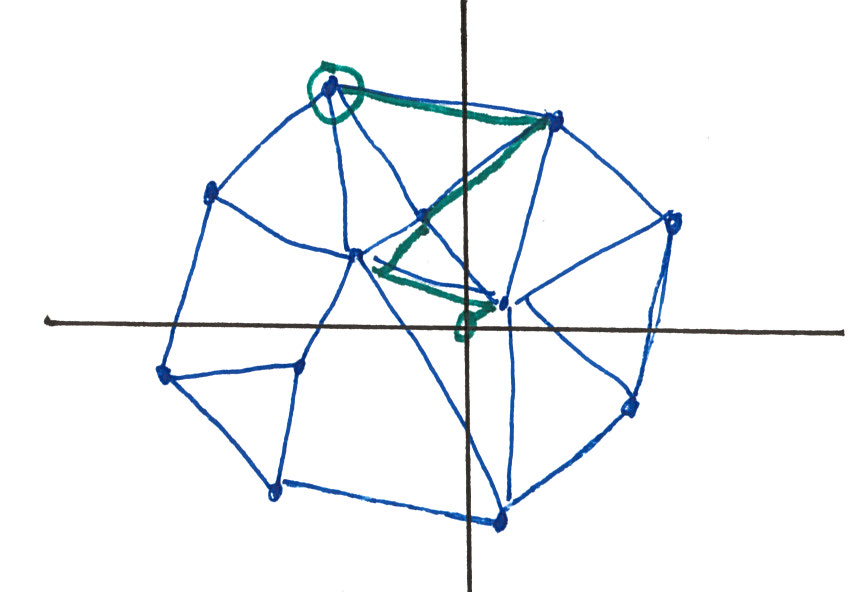
\includegraphics[width=2in]{simplex-solution.png}
  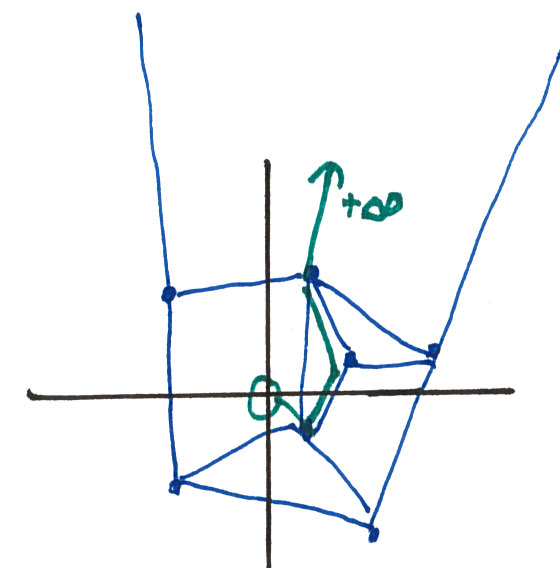
\includegraphics[width=2in]{simplex-unbounded.png}
\end{center}
\end{frame}

\begin{frame} \frametitle{Analysis}
  \begin{itemize}
    \item in LP's formulated to solve practical problems, usually
    \begin{itemize}
      \item each of the $m$ halfspaces intersects $O(m)$ other
        halfspaces
      \item $\Rightarrow O(m^2)$ intersection points in the feasible region
      \item $\Rightarrow$ simplex iterates $O(m^2)$ times
      \item each iteration involves evaluating $n$-dimension obj. function
      \item $\Rightarrow O(m^2 n)$ worst-case time
      \item order-3 polynomial, same as max-flow
      \item often faster b/c each step can ``jump'' pretty far
    \end{itemize}
    \item \textbf{however,} $\exists$ feasible LP's that force simplex to take
      $\Omega(2^m)$ time
    \item \emph{Klee-Minty cube:} $\forall d$, has $n=d$ variables, $n=d$ constraints,
      $2^d$ vertices, simplex is ``tricked'' into visiting all vertices
    \item this is a rare example of worst-case asymptotic analysis being misleading
    \end{itemize}
\end{frame}

\begin{frame} \frametitle{Klee-Minty Cube}
\begin{center}
  Klee-Minty Cube in 3D:

  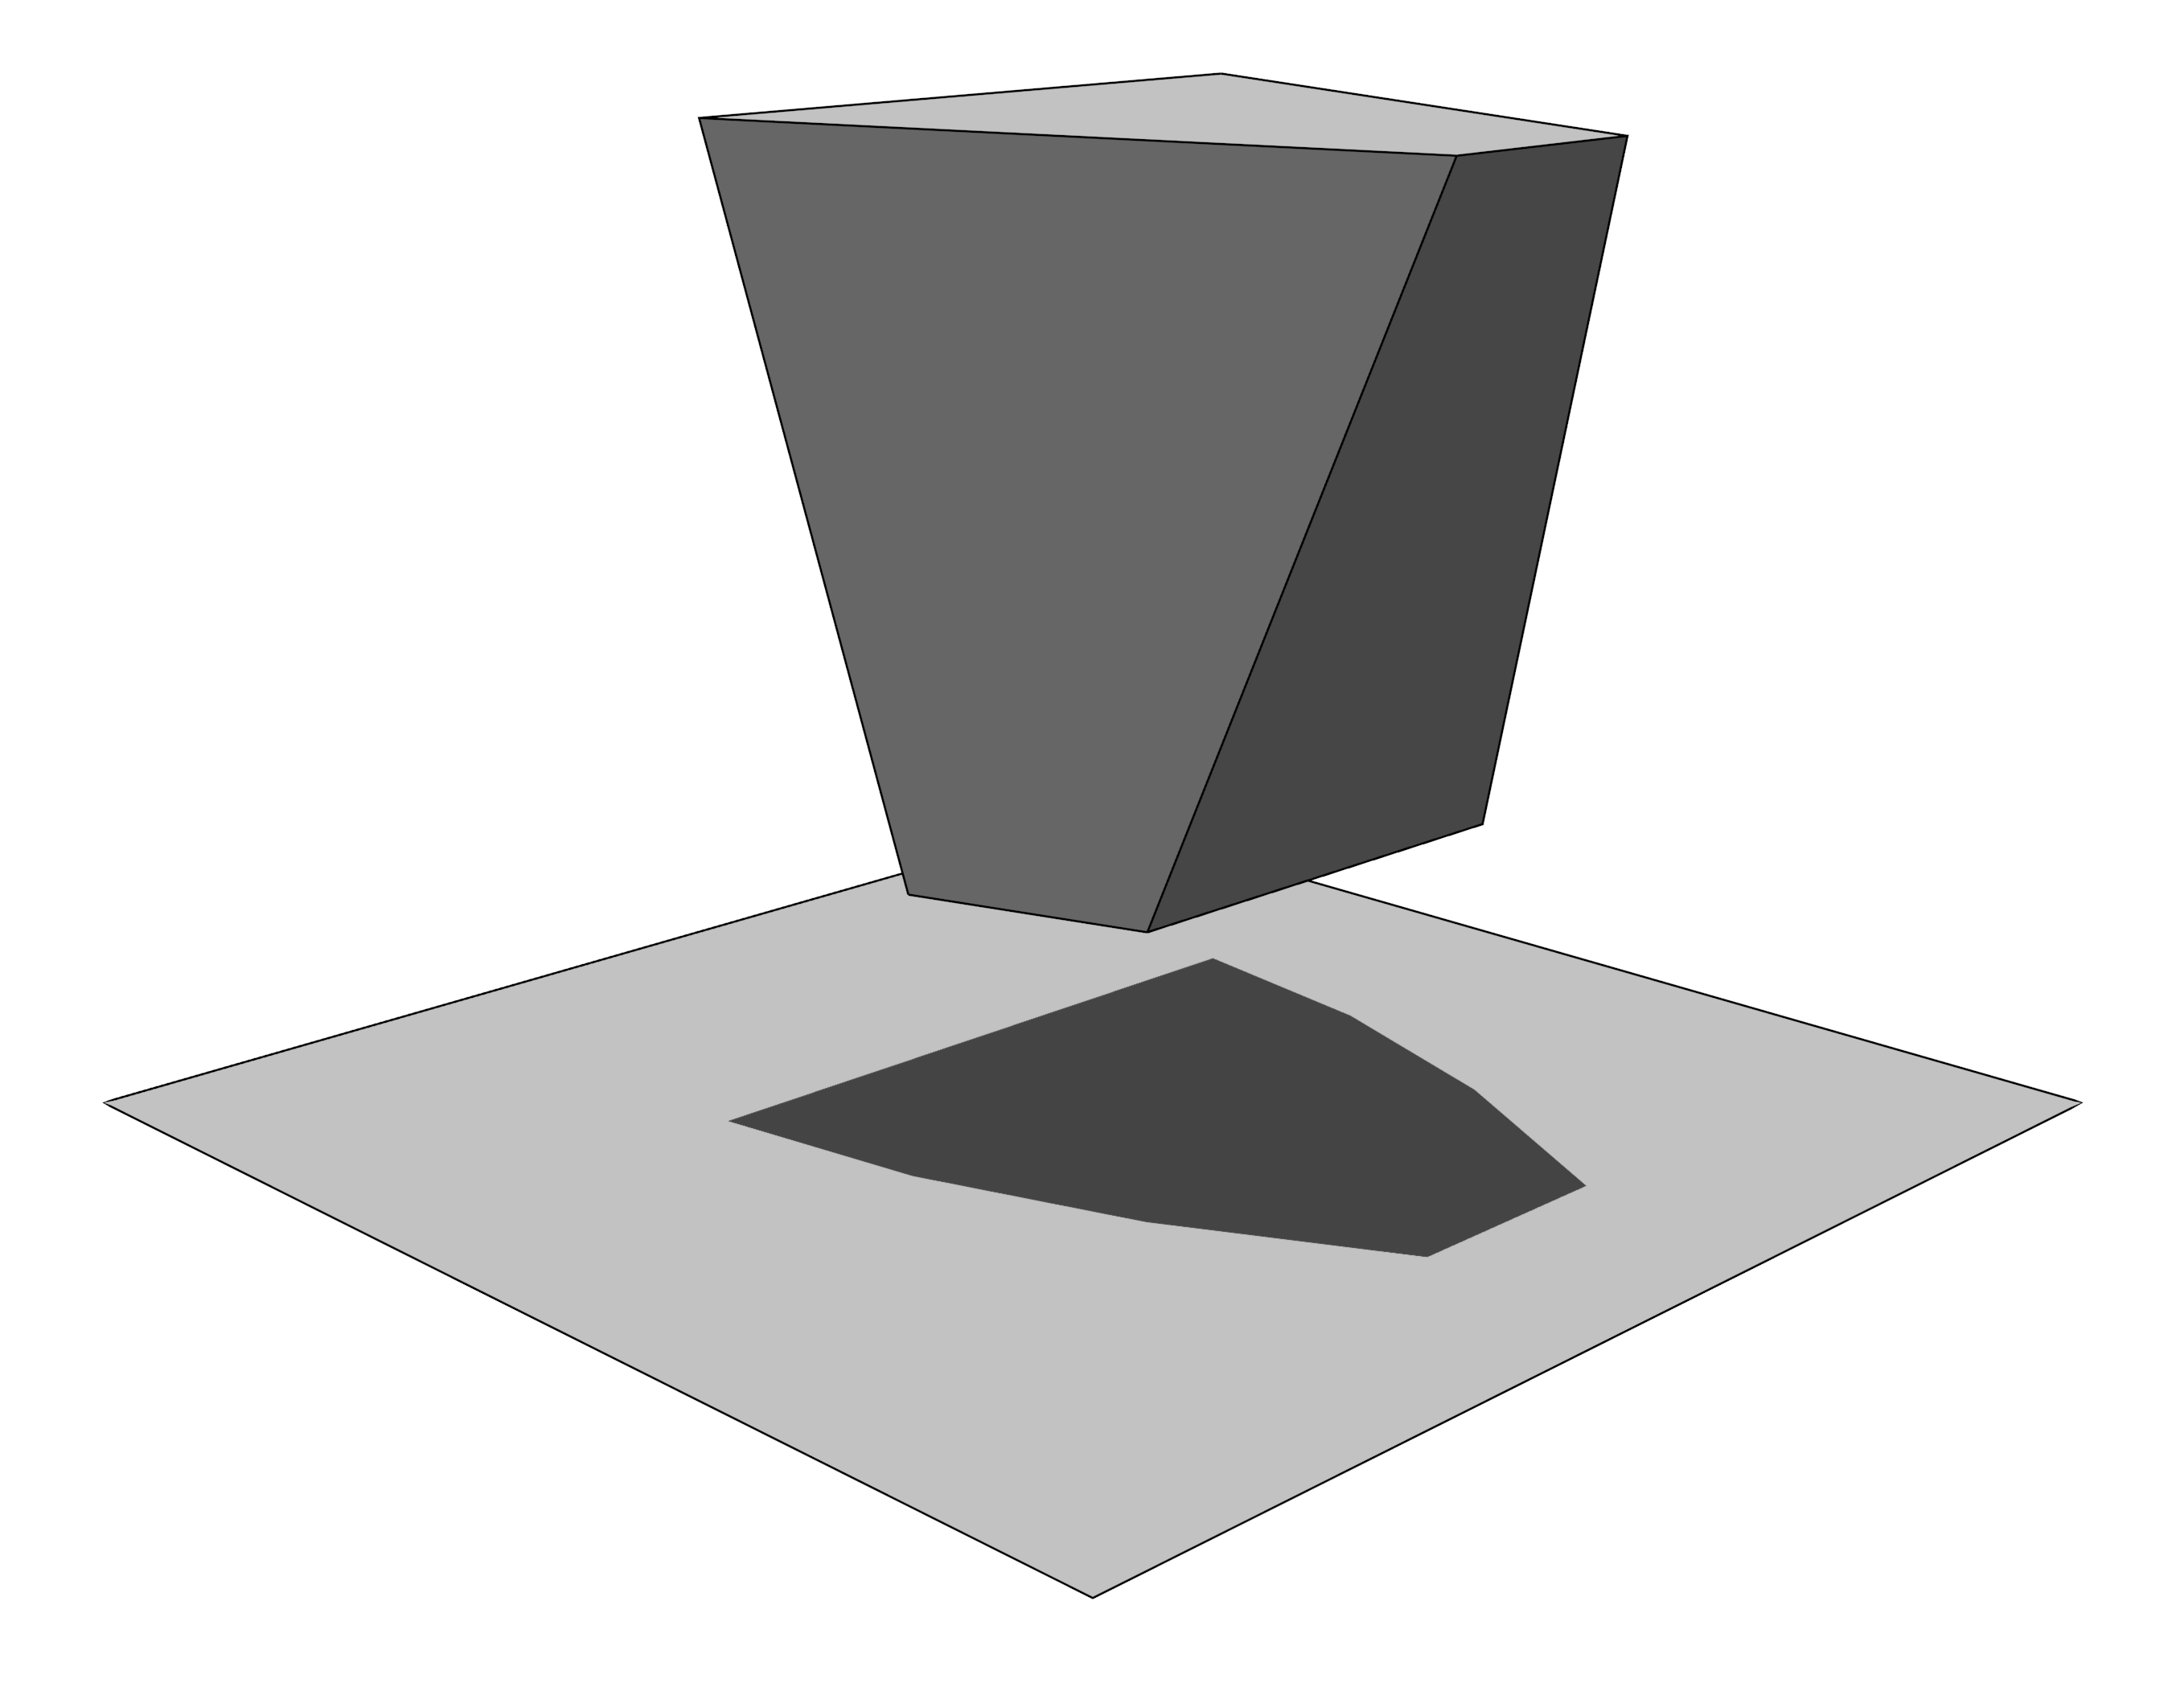
\includegraphics[scale=.07]{Klee-Minty-cube-for-shadow-vertex-pivot-rule.png}

  {\tiny
  (image credit: Sophie Huiberts, CC-BY 4.0, \url{https://commons.wikimedia.org/wiki/File:Klee-Minty-cube-for-shadow-vertex-pivot-rule.png})
  }
\end{center}
\end{frame}

\begin{frame} \frametitle{Summary}
  \begin{itemize}
    \item for a standard-form LP with $n$ variables and $m$ constraints...
    \item simplex algorithm is fast in practice, technically takes $O(2^m)$
      worst-case time
    \item Khachiyan's \emph{ellipsoid algorithm} takes $O(n^4 W)$ time
      \begin{itemize}
        \item seminal result, proved that sub-exponential algorithms are possible
      \end{itemize}
    \item now have faster pseudopolynomial algorithms, e.g Vaidya's alg.
      takes $O((n+m)^{1.5} nW )$ time
    \item open questions:
    \begin{itemize}
      \item Is there a strongly-polynomial algorithm, or is
      $LP$ $NP$-complete?
      \item Is there an algorithm that has \textbf{both}
      simplex' practical speed \textbf{and} provable pseudonomial runtime?
    \end{itemize}
  \end{itemize}
\end{frame}

\end{document}
